%%
%% This is file `sample-lualatex.tex',
%% generated with the docstrip utility.
%%
%% The original source files were:
%%
%% samples.dtx  (with options: `sigconf')
%% 
%% IMPORTANT NOTICE:
%% 
%% For the copyright see the source file.
%% 
%% Any modified versions of this file must be renamed
%% with new filenames distinct from sample-lualatex.tex.
%% 
%% For distribution of the original source see the terms
%% for copying and modification in the file samples.dtx.
%% 
%% This generated file may be distributed as long as the
%% original source files, as listed above, are part of the
%% same distribution. (The sources need not necessarily be
%% in the same archive or directory.)
%%
%% The first command in your LaTeX source must be the \documentclass command.
\documentclass[sigconf, nonacm=true]{acmart}
%% NOTE that a single column version may be required for 
%% submission and peer review. This can be done by changing
%% the \doucmentclass[...]{acmart} in this template to 
%% \documentclass[manuscript,screen]{acmart}
%% 
%% To ensure 100% compatibility, please check the white list of
%% approved LaTeX packages to be used with the Master Article Template at
%% https://www.acm.org/publications/taps/whitelist-of-latex-packages 
%% before creating your document. The white list page provides 
%% information on how to submit additional LaTeX packages for 
%% review and adoption.
%% Fonts used in the template cannot be substituted; margin 
%% adjustments are not allowed.
%%
%%
%% \BibTeX command to typeset BibTeX logo in the docs

\usepackage{graphicx}
\usepackage{float}

\AtBeginDocument{%
  \providecommand\BibTeX{{%
    \normalfont B\kern-0.5em{\scshape i\kern-0.25em b}\kern-0.8em\TeX}}}

%% Rights management information.  This information is sent to you
%% when you complete the rights form.  These commands have SAMPLE
%% values in them; it is your responsibility as an author to replace
%% the commands and values with those provided to you when you
%% complete the rights form.
\setcopyright{acmcopyright}
\copyrightyear{2018}
\acmYear{2018}
\acmDOI{10.1145/1122445.1122456}

%% These commands are for a PROCEEDINGS abstract or paper.
\acmConference[Woodstock '18]{Woodstock '18: ACM Symposium on Neural
  Gaze Detection}{June 03--05, 2018}{Woodstock, NY}
\acmBooktitle{Woodstock '18: ACM Symposium on Neural Gaze Detection,
  June 03--05, 2018, Woodstock, NY}
\acmPrice{15.00}
\acmISBN{978-1-4503-XXXX-X/18/06}

%%
%% Submission ID.
%% Use this when submitting an article to a sponsored event. You'll
%% receive a unique submission ID from the organizers
%% of the event, and this ID should be used as the parameter to this command.
%%\acmSubmissionID{123-A56-BU3}

%%
%% The majority of ACM publications use numbered citations and
%% references.  The command \citestyle{authoryear} switches to the
%% "author year" style.
%%
%% If you are preparing content for an event
%% sponsored by ACM SIGGRAPH, you must use the "author year" style of
%% citations and references.
%% Uncommenting
%% the next command will enable that style.
%%\citestyle{acmauthoryear}

\graphicspath{ {./images/} }

%%
%% end of the preamble, start of the body of the document source.
\begin{document}

%%
%% The "title" command has an optional parameter,
%% allowing the author to define a "short title" to be used in page headers.
\title{Ad-hoc Document Re-ranking by Query Attention and Document-level Context}

%%
%% The "author" command and its associated commands are used to define
%% the authors and their affiliations.
%% Of note is the shared affiliation of the first two authors, and the
%% "authornote" and "authornotemark" commands
%% used to denote shared contribution to the research.
\author{Sanchit Nevgi}
\email{snevgi@umass.edu}
\affiliation{%
  \institution{University of Massachusetts, Amherst}
}

%%
%% By default, the full list of authors will be used in the page
%% headers. Often, this list is too long, and will overlap
%% other information printed in the page headers. This command allows
%% the author to define a more concise list
%% of authors' names for this purpose.
\renewcommand{\shortauthors}{Nevgi et al.}

%%
%% The abstract is a short summary of the work to be presented in the
%% article.

\begin{abstract}
  Transformer-based models have recently been applied to the ad-hoc document ranking task, where they have outperformed other neural models such as KNRM \cite{Xiong2017EndtoEndNA}, PACRR \cite{Yang2017AnseriniET} and other traditional IR methods. However, Transformer-based models have a severe limitation that prevent them from being applied as-is to full documents, resulting in using paragraph-level workarounds. Using paragraphs scores may not perform well for documents which have information spread across paragraphs. The recently proposed Longformer model \cite{Beltagy2020LongformerTL} addresses the input size limitation. It handles long documents by using a combination of a local sliding window attention and an end-task motivated global attention mechanism. In this work, we apply the Longformer architecture in the document re-ranking task. Our hypothesis is that the local attention effectively captures the document representation, while the global attention on the query tokens aids in matching. Our code is made publicly available here \footnote{\href{github.com/sanchitnevgi/adhoc-ranking}{https://github.com/sanchitnevgi/adhoc-ranking}}
\end{abstract}

%%
%% This command processes the author and affiliation and title
%% information and builds the first part of the formatted document.
\maketitle

\section{Introduction}

Ad-hoc ranking over a large data regime is a fundamental task in Information Retrieval. It reflects common real-world web search scenarios. Formally, in ad-hoc retrieval, given a Query $Q$ represented by terms $\{ q_1, q_2, ... q_{|Q|} \}$ and a document D given by $\{ d_1, d_2, ... d_{|D|} \}$, the task is to compute $score(Q, D) = sim(Q, D)$ where $sim$ represents the similarity between the query and the document, which is then used to rank the documents. In most applications of IR, the collection may contain millions of documents and so the system must be reasonably efficient enough to handle such cases.

The TREC Deep Learning Track challenge was designed to test this very purpose. The challenge consists of two tasks --- (1) Document ranking and (2) Passage ranking task. In each task, participants can train models for full-ranking of the documents or use the provided top-1000  documents for re-ranking.

Nowadays, most practical IR systems have adopted a pipelined approach, where an initial set of candidates documents is obtained by statistical approaches such as BM25. The candidate set is then re-ranked to obtain the final rankings. To re-rank the candidate set, recent approaches have used neural methods such as Transformer models. However due to memory limitations of Transformer models, present techniques use paragraph-level workarounds to generate the document relevancy score.

However, the efficacy of these approaches poses several questions. The information that satisfies the user need could potentially be split across many paragraphs and the model would need document-level training signals to effectively capture relevancy.

In this project, we seek to incorporate document-level context in training neural models to obtain a better document ranking. To achieve this, we explore the approaches briefly listed below

\begin{enumerate}
  \item A recently proposed model known as Longformer \cite{Beltagy2020LongformerTL} makes use of global and local attention to obtain a representation of long documents. It has outperformed previous neural models in question answering domain. However, to the best of our knowledge it's performance in IR application is as yet untested. In this work, we propose using this model to obtain a representation of the document and get a matching score with the query.
  \item Transformer models have pushed the state-of-the-art in abstractive summarization tasks. In this approach, we train a model to generate document summary ("conditioned" on the query), with the intuition that this summary would closely reflect the user query. Next, we can conventional matching techniques to obtain a score for the re-phrased document query pair.
\end{enumerate}

The paper is organized as follows; \S \ref{related-work} describes the recent applications of neural networks, particularly Transformers, to large-scale document retrieval and ranking. \S \ref{background} describes the LongFormer architecture and how it applies to the document ranking problem. \S \ref{dataset} and \S \ref{baseline} describes the TREC DLT dataset and our baselines respectively. \S \ref{experiments} outlines our method and experiments and \S \ref{results} describes the results.

\section{Related Work} \label{related-work}

\textbf{Neural models.} With advancements in Deep Learning, neural models such as DRMM \cite{Guo2016ADR}, (Co)-PACRR \cite{Hui2017PACRRAP,Hui2018CoPACRRAC}, (Conv)-KNRM \cite{Xiong2017EndtoEndNA, Xiong2017ConvolutionalNN} have shown improved performance over traditional IR approaches in the document ranking domain.

\smallskip

\noindent \textbf{Transformer architectures.} There is an increasing trend towards using Transformer architectures \cite{Vaswani2017AttentionIA} such as BERT \cite{Devlin2019BERTPO} to re-rank documents from a candidate set. \citeauthor{MacAvaney2019CEDRCE} incorporated the contextualized word embeddings produced by BERT in existing neural IR architectures like the aforementioned PACRR and KNRM. \citeauthor{nogueira_passage_2020, yang_simple_2019} proposes a method to obtain document relevance score by aggregating over individual passage scores of the document. The passage score is obtained by computing the similarity between query and passage representation. The aggregated score is usually computed by taking a max or average over the paragraph scores.

\smallskip

\begin{figure*}
  \caption{The attention patterns of the LongFormer model. In our experiments, we globally attend to the query tokens. Image credit: "Longformer: The Long-Document Transformer"}
  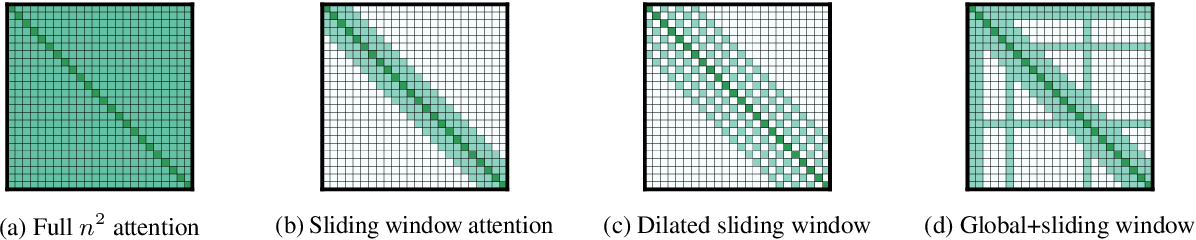
\includegraphics[width=\textwidth]{./images/longformer-attention.png}
  \label{fig:attention}
\end{figure*}


\noindent \textbf{Using Document context.} There has been limited work on using the entire document context in ranking documents, due to the memory constraints of Transformer models.The time complexity scales quadratically in proportion to the sequence length leading to using paragraph-level workarounds. This is a severe limitation as the information could be spread across paragraphs. 

\citeauthor{Li2020PARADEPR} introduce an end-to-end Transformer model that incorporates document-level context by evaluating BERT over a sliding window of words and concatenating the paragraph-level \texttt{[CLS]} tokens to obtain a document representation. An additional (smaller) Transformer model is applied to this representation, which supposedly incorporates the ordering and dependencies between passages.

Recently, \citeauthor{Beltagy2020LongformerTL} have proposed the Longformer architectures that uses a local windowed attention combined with a task motivated global attention. This architecture has shown promise in long document classification and question answering tasks. Figure \ref{fig:attention} shows the the attention pattern of the Longformer model. Note that the computation scales linearly with the input size instead of quadratically. In our approach, we globally attend to the query tokens.

\begin{table}[!h]
  \caption{Document length statistics from a representative sample ($n=1000$) of the dataset}
  \label{doc-length}
  \begin{tabular}{lrr}
    \toprule
    Statistic & Query Length & Document Length \\
    \midrule
    mean  &  31.09 &   8520.32 \\
    std   &  11.62 &  14472.29 \\
    min   &  10.00 &      8.00 \\
    25\%   &  23.00 &   2114.25 \\
    50\%   &  30.00 &   3963.50 \\
    75\%   &  37.00 &   8204.50 \\
    max   & 148.00 & 125199.00 \\
  \bottomrule
  \end{tabular}
\end{table}

\begin{table*}[!htb]
  \caption{Summary of statistics of TREC 2019 DLT challenge. The statistics are reproduced here verbatim \cite{Craswell2020OverviewOT}}
  \label{datastats}
  \begin{tabular}{l*4r}
    \toprule
    & \multicolumn{2}{c}{\textbf{Document Retreival Dataset}} & \multicolumn{2}{c}{\textbf{Passage Retreival Dataset}} \\
    \textbf{File Description} & Number of records & File size & Number of records & File size \\
    \midrule
    Collection & 3,213,835 & 22 GB & 8,841,823 & 2.9 GB \\
    Train queries & 367,013 & 15 MB & 502,940 & 19.7 MB\\
    Train qrels & 384,597 & 7.6 MB & 532,761 &  10.1 MB \\
    Validation queries  & 5,193 & 216 KB & 12,665 & 545 KB \\
    Validation qrels    & 519,300 & 27 MB & 59,273 & 1.1 MB \\
    Test queries        & 200 & 12 KB & 200 & 12 KB \\
  \bottomrule
\end{tabular}
\end{table*}

\begin{table*}[!htb]
  \caption{Summary of baseline results on the TREC DLT 2019 corpus using a fine-tuned BM25 model (with and without relevance feedback).}
  \label{baseline-stats}
  \begin{tabular}{rrrrr}
    \toprule
    & MAP & NDCG@10 & R@100 & RR  \\
    \midrule
    \textbf{BM25 (Fine-tuned)} & 0.3138 & 0.5140 & 0.3862  & 0.8872 \\
    \textbf{\;\; + RM3} & 0.3697 & 0.5485 & 0.4193 & 0.8074 \\
    $\textbf{BERT}_{passage}$ \cite{Chen2019UCASAT} & - &  \textbf{0.6437} & - & 0.8992 \\
    Longformer Base (ours) & \textbf{0.4353} & 0.6418 &  & \textbf{0.9011} \\
    \bottomrule
  \end{tabular}
\end{table*}

\section{Longformer architecture} \label{background}

\textbf{Sliding Window}: \cite{Beltagy2020LongformerTL}. \citeauthor{Kovaleva2019RevealingTD} show that local context contributes to the Transformers success. With this in mind, the LongFormer model applies a sliding window over the input. Formally, in a fixed window size $w$, the attention mechanism attends to $\frac{1}{2} w$ tokens on either side. Further, multiple stacked layers of this sliding window is applied to obtain the input representation. Figure \ref{fig:attention}, shows the various attention mechanism. In our case, the sliding window obtains a document representation. Further work is needed to justify if the obtained document representation is better compared to prior work. \\

\smallskip

\noindent \textbf{Global Attention}: For many tasks, the local context isn't sufficient to obtain a good model. For example, question answering tasks require the model to pay attention to the question to highlight the relevant spans in the provided context. The Longformer adds a symmetric global attention mechanism. Traditional attention mechanism \cite{Vaswani2017AttentionIA} are computed as;

\begin{equation}
  \text{Attention}(Q, K, V) = \text{softmax}\left( \frac{QK^T}{\sqrt{d_k}}\right) V
\end{equation}

The Longformer uses 2 sets of projection for local and global attention. $Q_i, K_i, V_i$ for $i \in \{ l, g\}$

\section{Dataset} \label{dataset}

We use the data provided for the TREC DLT 2019 challenge. It comprises of a large human-generated set of training labels from the MS-MARCO dataset \cite{Campos2016MSMA} with additional relevance judgement from NIST assessors.

The documents were judged on a four-point scale of Not Relevant (0), Relevant (1), Highly Relevant (2) and Perfect (3). The For binary relevance judgements, the levels 1--3 are considered to be \textit{relevant} and level 0 is deemed \textit{not relevant}.

Table \ref{datastats} lists the TREC DLT dataset statistics. Note that in this work, we solely focus on the document retrieval dataset. Table \ref{doc-length} lists the document and query length statistics. This helps us select the input sequence length for our model as described in \S \ref{experiments}.

\section{Baseline} \label{baseline}

For our baselines, we implemented a fine-tuned BM25 model using the Anserini toolkit \cite{Yang2018AnseriniRR}. Anserini is an open-source toolkit built on Lucence \cite{Yang2017AnseriniET} with the goal to enable reproducible baselines for academic as well as real-world Information Retrieval applications \cite{10.1145/3239571}.

Using Anserini, we index the TREC 2019 corpus with the default settings, which uses the Porter stemmer. Next, we perform retrieval on the index using the fine-tuned BM25 model which is configured with $k1 = 3.44$ and $b = 0.87$. Additionally, we also use the RM3 re-ranker with 10 feedback documents and queries. The original query is given a weight of $0.5$.

The BM25 model with Relevance Feedback (RM3) outperforms the fine-tuned BM25 in MAP and nDCG metrics. Since these metrics are the most relevant to us, we compare our approach to the this model going ahead.

The summary of our baseline results are provided in Table \ref{baseline-stats}.

\section{Evaluation} \label{evaluation}

We evaluate our model using the Mean Average Precision (MAP) and Normalized Discounted Cumulative Gain (nDCG) and Mean Reciprocal rank (RR) metrics. This is in line with the metrics used for the TREC DLT 2019 challenge \cite{Craswell2020OverviewOT}. These metrics were chosen to reflect the performance of real-world search engines, where a majority of queries return multiple relevant documents. Our model is evaluated on the official query test set, which consists of 200 queries and a ranked list of the top 100 documents and their relevancy scores.

\section{Experimental Setup} \label{experiments}

In modern applications of document information retrieval, the corpus size is very large (in the order of billions). To combat this, practitioners use a pipelined approach. An initial set of 100 documents is retrieved with traditional IR methods such as BM25. Subsequently, we use a neural model to re-rank the candidate set to get final rankings. The TREC dataset provides a candidate set, retrieved with a fine-tuned BM25 similar to the approach describes in \S \ref{baseline}.

As mentioned previously, we use the Anserini toolkit for our baselines. For our main approach, we make use of the \texttt{PyTorch}'s \footnote{\href{https://pytorch.org/}{https://pytorch.org/}}auto-differentiation mechanics and the \texttt{transformers} \footnote{\href{https://github.com/huggingface/transformers}{https://github.com/huggingface/transformers}} library to build and train our model. We evaluate our results using the \texttt{trec\_eval} tool provided by Anserini. 

\medskip

\noindent \textbf{Dataset Pre-processing}: We generate a 10,000 training and 1,000 dev triples from the provided training and dev dataset, using the script \footnote{\texttt{msmarco-doctriples.py}} from the TREC DLT repository. Each triple consists of $(q, d_{pos}, d_{neg})$, where $q$ is the query, $d_{pos}$ is a positively judged document and $d_{neg}$ is any other document, randomly picked from the initial candidate set. Using this we create a positive and a negative query-document pair resulting in 20,000 training examples.

In our approach, we use a \texttt{longformer-base} model with a linear layer on top of the classification token (\texttt{<s>}) for binary classification (relevant or non-relevant). The model was pre-trained on long documents using the MLM objective \cite{Devlin2019BERTPO}. The input is a concatenated query-document pair, separated by a delimiter token and tokenized using the byte-level Byte-Pair-Encoding \cite{Liu2019RoBERTaAR} as shown below.

\begin{quote}
  \texttt{<s> query </s> document </s>}
\end{quote}

In addition, we build a global attention mask that attends only to the query tokens.

\smallskip

\noindent \textbf{Model configuration}: We use a $seq\_len \in \{4000, 10000\}$ as it effectively captures 50\% and 80\% of the corpus without truncation as seen from Table \ref{doc-length}. As expected, a longer sequence length performs better due to the longer context. Additionally, we use the GeLU non-linearity and 12 hidden layers and attention heads.

\smallskip

\noindent \textbf{Training}: We use the Adam optimizer \cite{Kingma2015AdamAM} with a learning rate of $3e-5$. The pre-trained Longformer model is fine-tuned on an NVIDIA 2080-ti GPU for a maximum of 10000 steps. We also experiment with a learning rate schedule with a linear warmup for 200 steps. However, we found that it leads to a slower convergence and doesn't improve performance significantly. Due to the large input size, we use a batch size of 2 and accumulate gradients for 4 batches, leading to an effective batch size of 8. We also train on half precision to speed up training. The results of our experiments are shown in Table \ref{baseline}.

\section{Results \& Analysis} \label{results}

In this work, we seek to improve the document re-ranking in a large data regime as put forth by the TREC DLT 2019 challenge. We do so by leveraging the LongFormer's local sliding window attention mechanism while globally attending to the query tokens to obtain a document relevancy score. We find that by globally attending to the query tokens the model is able to create a better representation of the document without having to use paragraph-level workarounds. Our approach using the Longformer-base model outperforms the baseline fine-tuned BM25 methods as measured by the nDCG, AP metrics and is comparable to the recent BERT models that have specialized architectures to utilize passage-level representations.

\section*{\small{Team Members and Overlap statement}}

This is an \textbf{individual} project, inspired from the \textbf{default} "Ad-hoc ranking" project specification. It \textit{does not overlap} with any of the author's current or previous work.

\bibliographystyle{ACM-Reference-Format}
\bibliography{milestone}

\end{document}
\endinput
